\chapter{Análisis y Diseño}
    \par Cómo se ha expresado, la tarea de la mesa de ayuda es actualmente ayudar a responder las inquietudes de los alumnos, con foco en las preguntas más frecuentes. Esto con el fin de mejorar el viaje por los procesos académicos, sobre todo mejorando la comunicación entre las diversas fuentes de información y el alumno. Esto ayuda a disminuir la ansiedad, a mejorar los tiempos de respuesta y escalar en la cantidad de alumnos que se puede atender. Este proyecto no solo abarca las preguntas frecuentes, sino que establece una comunicación con actores reales de ser necesario, además de fomentar la centralidad de la información para el alumno, y de esa forma establece como paradigma general, acompañar al estudiante de forma eficaz. Por ende, pretende ser una plataforma que se pueda consultar de forma genérica, ayudando a resolver la mayoría de las inquietudes de los alumnos, priorizando la información que requiere ser contestada por autoridades oficiales y así disminuyendo la carga sobre todo en las preguntas frecuentes que cada funcionario debe responder.
    \par Hay variados desafíos en torno al diseño del sistema, la implementación y uso del mismo. Una de las grandes preocupaciones al desarrollar el sistema, era diseñar una infraestructura tanto lógica como de software, que permitiera abarcar no solo las necesidades de los alumnos, sino también la manera en que ellos esperan que estas necesidades sean resueltas. Ya que esto es un elemento clave en la adopción de tecnologías como los chatbots (). Además de ser el paradigma central de \acrlong{UCD}
    \par Para ello el proceso de análisis y diseño tomó como input las valoraciones de: los alumnos, potenciales usuarios del sistema, o de exalumnos \footnote{Usuarios que ya hubieran pasado por la mayoría de los procesos académicos de pregrado}. Y partir de estos resultados, se esquematizan sus necesidades para  desarrollar manteniendo no solo las funcionalidades y contenidos deseados, sino también la manera en que se quieren obtener los resultados.
    \par Entonces, para lograr este diseño holístico se realizaron: Dos Focus Groups (su metodología y resultados se detallan a continuación), un diseño basado en i* de necesidades y objetivos, y un diseño basado en UML para la capa de software. Además se llevó a cabo un proceso de refactoring del código del bot para: ser extensible, aceptar nuevas funcionalidades y separar las capas lógicas de la solución.

\section{Exploración a través de Focus Groups}
    \par Una de las problemáticas del trabajo realizado, era validar con usuarios del \acrshort{dcc} las propuestas obtenidas de la investigación teórica. Con el fin de recoger sus preferencias de manera explícita en la interacción con el sistema. Para esto, se llevaron a cabo dos \textit{\acrlong{f}}. En ellos se realizaron consultas en torno a la información a la que se puede y podría eventualmente acceder a través del bot, información sugerida a través del comportamiento social, el acompañamiento de terceros, la motivación para obviar el contacto directo con personas, privacidad y opciones de notificación.
    
    \subsection{Caracterización de los participantes}
    \par Los participantes del primer \acrshort{f}, son alumnos y ex-alumnos del \acrshort{dcc}. De estos, ocho de los nueve han presentado problemas relativos a información académica, es decir, la falta de información o información errónea les ha dificultado el avance en algunos procesos académicos. Cinco de nueve, no han cursado ningún ramo relativo a la memoria, sin embargo, todos han participado de procesos con plazos como las prácticas profesionales o \acrlong{ps}. En el caso del segundo \acrlong{f} las características son similares, pero son solo cuatro alumnos. Adicionalmente se llevaron a cabo conversaciones con el \acrshort{cadcc}, para evaluar las temáticas, respuestas y soluciones alternativas al sistema.
    
    \subsection{Respuestas de los estudiantes}
    \par A continuación, se detallan los resultados obtenidos para las categorías anteriormente descritas. Lo obtenido en cada consulta, se muestra de forma conjunta para ambos \textit{\acrlong{f}}, con el fin de analizar los mismos tópicos de forma única. Por lo tanto, de aquí en adelante cuando refiramos este término (\acrlong{f}) nos estaremos refiriendo al proceso de consulta completo.
    
    \begin{itemize}
        \item \textbf{Información a la que se puede acceder a través del bot:} El contenido al que se puede acceder actualmente a través del bot, son solamente las preguntas frecuentes. En relación con las nuevas funcionalidades de suscripción se les preguntó a los estudiantes cuál era la información relevante para ellos, sobre qué cosas querían un recordatorio o sugerencias.
        \par La mayoría está de acuerdo en que las fechas, ya sean de apertura o cierre de procesos, incluso tareas o avances parciales serían un contenido que ellos desearían del bot, cómo una notificación. También los cambios en la información relativa a un proceso, se deberían comunicar oportunamente, por otro lado, no se debería notificar un cambio de plazo, sino ajustar los recordatorios a los nuevos plazos. Cómo sugerencias, se admiten temas relacionados con los procesos en los que se esté suscrito o se haya preguntado reiteradamente ya sea por parte del usuario o por usuarios \guillemotleft similares\guillemotright.
        \par Aparte de las notificaciones, se sugirió dar acceso a información relevante del proceso en cuestión, tales como: el contacto público de personas relacionadas con el proceso \footnote{ejemplos serían: el correo el coordinador del \acrshort{e}, contacto de la secretaria docente, etc.} y ejemplos de válidos de los requisitos para cierta etapa (preinscripciones de práctica, ejemplos de propuestas de memoria).

        \item \textbf{Información Social:} Sobre este punto, la consulta era en torno a si estarían dispuestos a recibir sugerencias de contenido, a partir de otros usuarios con perfiles similares.
        Aquí las opiniones estaban divididas. Aunque en el alumnado se es reticente a compartir información con terceros, no habría problemas en que fuera información exclusivamente académica, relacionada con fines laborales o información que otros organismos ya tengan.

        \item \textbf{Usuario de Apoyo:} La idea de esta pregunta, era saber qué tan dispuestos están en involucrar un tercer actor que pueda ser de ayuda en un proceso académico.  A este ente le denominaremos usuario de apoyo. El ejemplo, era que el profesor guía recibiera un aviso cuando el alumno no respondiera ni interactuara con el bot, durante el proceso de titulación. Las respuestas dan cuenta de que no hay un acuerdo claro en cuanto a esto. Para algunos era algo viable, para otros era algo opcional, mientras que unos pocos preferían descartar de plano la alternativa.
        \par Finalmente a pesar de los cuestionamientos a su funcionalidad y a la forma de usar los bots de cada alumno. Se pudo consensuar que: Fuera una opción habilitada por el usuario y con posibilidad de deshabilitar en cualquier momento, coloquialmente  \guillemotleft cómo hacer un sudo\guillemotright. Así mismo, los parámetros asociados a este tercero como el contacto e información a la que accede también deberían ser definidos por el usuario. De esta forma, se elige al usuario de apoyo que cada usuario decida y se asocia al aspecto que él decida.

        \item \textbf{Motivación para obviar el contacto:} Esta pregunta busca profundizar en las razones de por qué los alumnos podrían preferir el bot, por sobre contacto directo con otra persona. En este caso, las razones son diferentes para cada alumno, pero concuerdan con la literatura de lo que se busca en un sistema de información \cite{Thurman}. Algunas de ellas son: ansiedad producto de la interacción, para no molestar, porque las preguntas son repetitivas, algunas mejoras funcionales como la rapidez, sugerencias a temas que tal vez no surjan de una pregunta directa a un encargado humano, la libertad de acudir cuando se desee y la sensación de control sobre la interacción.
        
        \item \textbf{Privacidad:} Dentro de este ítem, se preguntó específicamente por la privacidad de la información que el bot pudiera almacenar, y que \textit{trade-off} estarían dispuestos a realizar por más funcionalidades. Aquí hay acuerdo en que debería ser la mínima información posible y en caso de ser más, solo información académica. Por otro lado, la mayoría estuvo de acuerdo en conceder permisos temporales y sin guardar información de forma permanente, en caso de que alguna funcionalidad requiera más información. De este modo se vuelve a repetir la configuración y permisos personalizados a cada alumno.
        
        \item \textbf{Opciones de notificación:} En el caso de las opciones de notificación, se puede observar que las notificaciones deberían ser: cortas con poca información y personalizables. Cada notificación debería mostrar: el área a la que pertenece o una forma de saber qué temática o relacionado con qué es esa notificación. Al mismo tiempo, debería ser capaz de explicar en breves líneas, que es la información nueva. En el caso de que se requiera más espacio o se necesite mostrar más contenido, debería agregarse un link o un enlace en el que se pueda desplegar a través de una página o un blog la información necesaria pero no directamente en el Chat.
        
    \end{itemize}

\subsection{Análisis y conclusiones}
    \par A pesar de que en el \acrlong{f} se puede ver una ligera tendencia a ciertas características a partir del grado de avance de los alumnos, en general lo que se puede observar es que no hay una correlación directa entre el grado de avance y las preferencias personales de cada alumno, así que se propone una caracterización alternativa, asociar a los estudiantes en tres grupos: Primero, aquellos que prefieren definir absolutamente todos los parámetros de su interacción. Segundo, los que prefieren que se les sugiera o lo que se les facilite la interacción. Tercero, sería el usuario mixto que prefiere cierto grado de personalización mientras que prefiere una simplificación de otras tareas.
    \par Generalmente los alumnos que prefieren una alta especificación o definir cada una de las características, están también ligados a un alto grado de valoración de la privacidad y configuración manual. Se perciben a ellos mismos como autosuficientes.
    \par Por otro lado, los alumnos que suelen tener un interés más práctico, valoran entablar la menor cantidad de interacciones posibles y valoran mucho más la eficiencia del flujo de trabajo y su tiempo. Generalmente se perciben a sí mismos como no tan atentos a las tareas y algo desconcentrados.
    \par A partir de esto, vamos a caracterizar los tres grupos de estudiantes con tres nombres: el primero se denomina un \acrfull{S}, el segundo vendría ser un \acrfull{R} y el tercero se nombra como un \acrfull{P}.
    \par También podemos caracterizar la forma en que persiguen sus objetivos, los distintos actores en el sistema, esta puede variar dependiendo del proceso en el que se esté, la experiencia previa y las preferencias personales. Cabe destacar que no responden específicamente las caracterizaciones de cada uno de los alumnos es decir un \acrshort{P} aun así puede querer valorar o perseguir la privacidad al consultar información y también un \acrshort{S} puede perseguir la funcionalidad de los recordatorios.
    \begin{figure}[h]
        \centering
        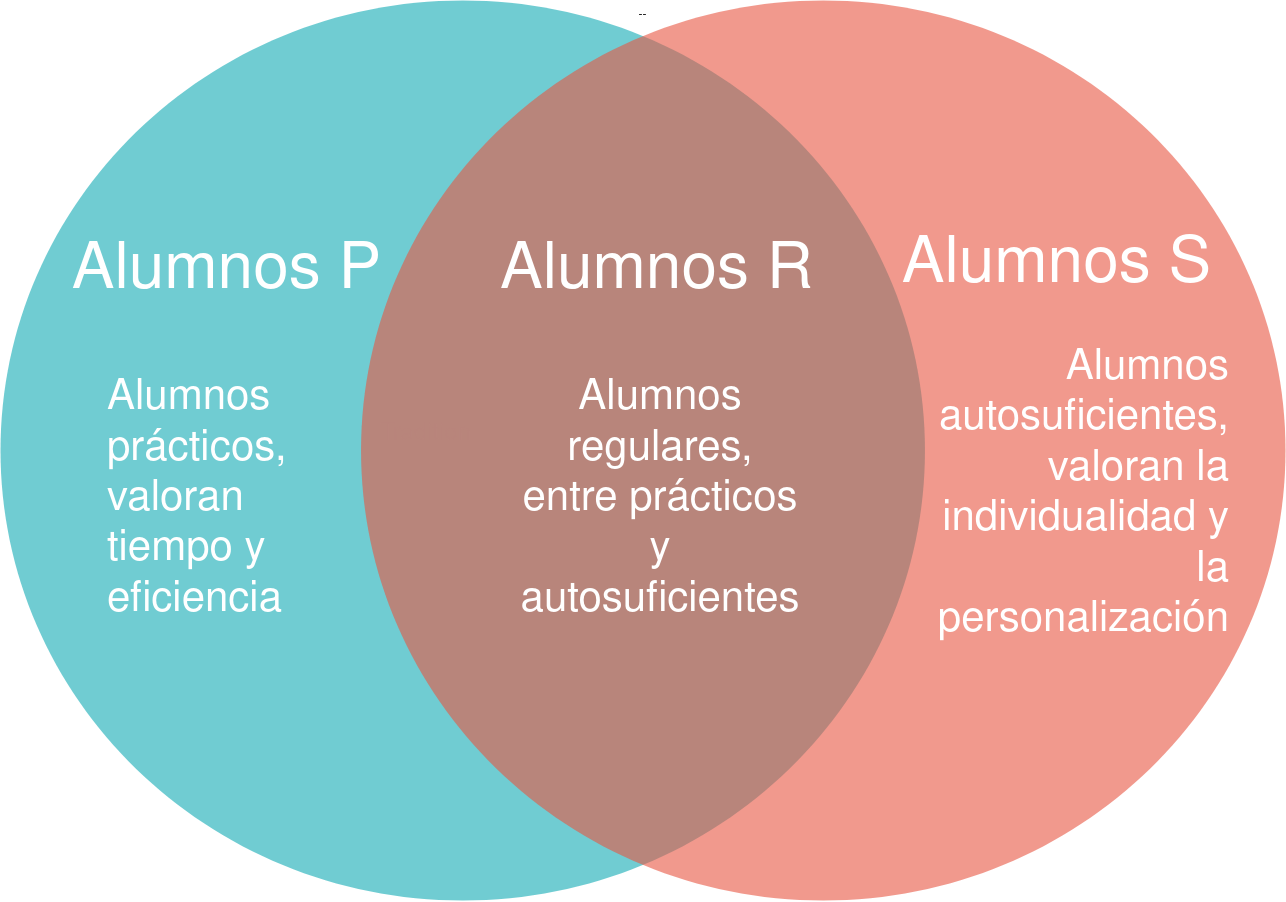
\includegraphics[scale=0.2]{media/imagenes/focus_groups/Tipos_de_alumnos-Diagrama_de_Venn.png}
        \caption{Diagrama de Venn: que representa los tipos de estudiantes encontrados en el \textit{Focus Group}.}
        \label{fig:alumnosVenn}
    \end{figure}
    \par Como conclusión se puede ver una tendencia a la personalización de la mayoría de los elementos funcionales, a sí mismo, una actitud selectiva en torno al contenido. En el caso de la privacidad, es más complejo. Se debería poder elegir tanto cuáles permisos son entregados y su duración. En el caso de las notificaciones, poder establecer su frecuencia en cualquier momento. En el caso de las sugerencias, se accede a entregar más información o recibir sugerencias siempre y cuando esto sea establecido por el usuario y que la información dada tenga el carácter de input temporal y no almacenado. Así mismo se establece que el usuario de apoyo debe ser definido por el estudiante. Todo esto va en línea con la investigación preliminar que sugiere que los usuarios valoran la personalización y lo relevante de la información para cada usuario suele ser completamente diferente. Todo lo anterior, hace que este trabajo esté orientado en la dirección de las necesidades y preferencias del estudiantado, al mismo tiempo que va en línea con los descubrimientos y los trabajos relacionados.

\subsection{Nuevos Modelos de Interacción}
    \par En esta sección se detalla las problemáticas de diseño de los nuevos modelos, luego se condensan los tipos de contenido que debería tener el sistema, las funcionalidades y las modalidades de interacción que surgen de las preferencias de los usuarios

    \subsubsection{Problemáticas de diseño de los nuevos modelos}
    \par A partir de la diversidad de opinión y de preferencia que se extrae de la investigación a través de \acrlong{f}, podemos ver que la complejidad del modelo subyacente a tales impresiones es alta. Por la misma razón, el sistema va a tener una manera diferente de concretar los objetivos de estos actores dependiendo de cuáles sean estos objetivos y cuáles sean las tareas o requisitos asociados a tales objetivos. A raíz de esto, se hace extremadamente necesario poder especificar con claridad cada uno de los requisitos y sin embargo poder englobarse en funcionalidades que respondan de manera unilateral a las necesidades de las personas, es decir a través de la misma interfaz, la del chatbot. Por eso es que antes de involucrarnos en el diseño funcional o computacional o generar algún diagrama como el de arquitectura o de clases. Se hace necesario plasmar de manera clara las diferentes necesidades de los alumnos en el sistema, las características de estos objetivos, sus relaciones y como pueden ser llevados a la concreción.
    
    \par Estas diferencias de parecer y de uso, hacen que el sistema a crear deba ser altamente configurable, es decir que cada usuario puede definir que quiere y cómo lo quiere. El cómo responder a las necesidades de los distintos usuarios determina las funcionalidades del sistema, así mismo el qué o la propia necesidad por un contenido específico determina cuál será la información del sistema. A partir de esto, podemos resumir lo que buscan los diferentes usuarios en el sistema en dos grandes categorías contenido, es decir fechas, definiciones, actores relacionados, requisitos, consecuencias, etc. y funcionalidades, tales como recordatorios, consultas, entre otros.
    \par Desde esta separación preliminar se proponen diferentes definiciones y diagramas, los que ayudan a encapsular y explicar de manera concisa y clara el modelo de interacción de alumnos y alumnas, sin perder el foco en los objetivos de los mismos.
    \par Para lograr esto se propone la adopción de la simbología del lenguaje gráfico \gls{i*} \cite{Dalpiaz2016}, con el fin expresar de forma correcta a los actores involucrados, sus preferencias y asimismo las tareas subyacentes que el sistema debería realizar para completar los objetivos que cada uno de estos actores tiene.
    \par A partir de la investigación del estado del arte, la exploración a través de \textit{focus groups} y el análisis posterior, se define lo siguiente:
    
    \subsubsection{Contenidos del Sistema}
    \label{sssec:contenidos}
    \par Los contenidos que buscan los alumnos a través del bot los podemos agrupar en cuatro categorías Definiciones, Requisitos, Fechas y Actores.
    \par las Definiciones son la descripción o detalle del proceso, a grandes rasgos, es una explicación de se trata el proceso, como su nombre lo expresa muy bien, cumplen un rol \textit{educativo}, que es informar al usuario de que es lo que se trata este proceso. La idea de este tipo de información es que el usuario puede entender en una sola consulta que es el proceso, de que trata, que consigue con él, de forma eficiente y amigable.
    \par Los Requisitos son todas aquellas cosas que serán solicitadas durante el proceso, y que permiten el avance durante el mismo. El alumno busca enterarse de cuáles son estas cosas, que tareas o asignaciones debe realizar para lograrlo y ejemplos válidos de una tarea completada. Por ejemplo, un ejemplo de requisito para el proceso de práctica sería realizar la preinscripción de práctica. Al consultar en el sistema el alumno debería obtener el requisito junto a una explicación de en qué consiste y un ejemplo válido de cómo realizarla.
    \par Las fechas son todas aquellas fecha relevantes en un proceso, en general definen plazos o hitos durante el proceso. Por ejemplo la fecha de entrega del primer avance en el \acrshort{e}
    \par Los actores son todos aquellos entes relacionados con un proceso, tienen cuatro características que serían: el rol que cumplen dentro del proceso (el cargo o responsabilidad dentro del proceso), el contacto (medio para localizarlos), proveen de un servicio dentro del proceso (las tareas asignadas a su rol) y tendrían una asociación o un grupo al que pertenecen, por ejemplo dentro de una categoría "tipo profesor" este podría pertenece al rol de "Académicos" o "Universidad", mientras que una institución que provee de prácticas podría pertenecer a la categoría de "Externos" o "Lugares de práctica".
    \subsubsection{Funcionalidades relativas a la información}
    \par Las funcionalidades buscadas se puede agrupar también en 4 grupos: Consultas, Sugerencias, Intervenciones y Recordatorios.
    \par Las Consultas son un tipo de interacción ya presente y que consiste en acceder al bot para realizar alguna consulta sobre la información de un determinado proceso, esta información podría ser cualquiera de los contenidos listados arriba.
    \par Las Sugerencias son de un formato similar a las consultas, pero son entregadas sin ser solicitadas directamente, debe poder activarse y desactivarse, además de que no deben ser entregadas en cualquier momento, sino ojalá con una periodicidad predeterminada por el usuario, buscan ayudar al usuario a encontrar o enterarse de contenido que podría serle de utilidad sin ser buscado directamente, es decir a partir de su interacción y usuarios con características similares.
    \par Los recordatorios son un tipo especial de notificación que es gatillada expresamente por el usuario quien les fija una periodicidad o frecuencia, buscan ayudarlo a programar y efectuar los trabajos de manera efectiva. Tienen la opción de requerir feedback si el usuario así lo desea, para motivar el compromiso.
    \par Las intervenciones son habilitadas por el usuario y permiten al bot enviar notificaciones que alteren o podrían alterar el curso conocido del proceso, estas notificaciones pueden ser enviadas tanto al estudiante cómo al estudiante, cómo a un tercero que estudiante defina, en variados casos. Por ejemplos, los cambios en los requisitos serían una intervención, y esa modificación sería enviada al alumno. Por otro lado un cambio de fechas no siempre se categorizan como intervención, dependiendo del alumno, y del plazo. Por esta razón las intervenciones tienen un periodo de vigencia, en el que son relevantes y deberían proveer idealmente suficiente marco de acción para tomar medidas pertinentes al caso. También podrían ser provocadas por el estudiante al no responder a una interacción pactada como los recordatorios, siempre y cuando esto haya sido habilitado y parametrizado por el alumno.
    
    \subsubsection{Modalidades de Interacción}
    \label{sssec:cualidades}
    \par la mayoría de reticencias o preferencias de los alumnos, respecto a como se deben llevar a cabo las tareas asociadas a los objetivos de contenido o funcionalidad, se pueden agrupar en 5 categorías Privacidad, Parametrización, Eficiencia, Individualidad y Confiabilidad.
    \par la Privacidad hace referencia a la información que el alumno debe entregar para obtener cierta funcionalidad o contenido. En general se busca que exista la mayor privacidad posible, pero algunas interacciones contienen un \textit{trade-off} entre privacidad y eficiencia por ejemplo, que algunos alumnos están dispuestos a aceptar.
    \par La Parametrización tiene que ver con la configurabilidad de la funcionalidad en cuestión, dependiendo del estudiante es más o menos valorada, y esto implica que el sistema debe dar las opciones de parametrización al tiempo que simplificarlas dependiendo del alumno.
    \par La Eficiencia hace referencia a que tan bien puedo cumplir la tarea en cuestión, usualmente relacionada a obtener más recursos o simplificar las parametrizaciones de una funcionalidad determinada.
    \par La Individualidad propone la autonomía del usuario en esa funcionalidad, por ejemplo, buscar contenido de memoria o de práctica sin avisar a otros actores. O no avisar inmediatamente al profesor guía de una omisión sin que el alumno haya consentido esto.
    \par La Confiabilidad por último hace referencia tanto a la validez de la interacción como la confianza que alumno puede descargar en tal interacción. Por ejemplo, que los contactos consultados de un determinado actor estén vigentes.
    
    \subsubsection{Resumen conceptual del modo de Interacción}

    \par este resumen pretende expresar de manera breve, los diferentes contenidos, funcionalidades y modalidades a través de un diagrama jerárquico de clases o de conjuntos. Cómo se podrá observar más tarde en la sección \ref{}, las funcionalidades determinan de qué forma se quiere obtener un determinado recurso del sistema, son la interfaz funcional del sistema. Por otro lado los contenidos, son los datos que el sistema debe almacenar para posteriormente servir, estos a su vez definen modelos de datos de la información del sistema. Finalmente las Modalidades hacen eco de los valores presentados en la interacción alumno-bot.
    
    \begin{figure}[h!]
        \centering
        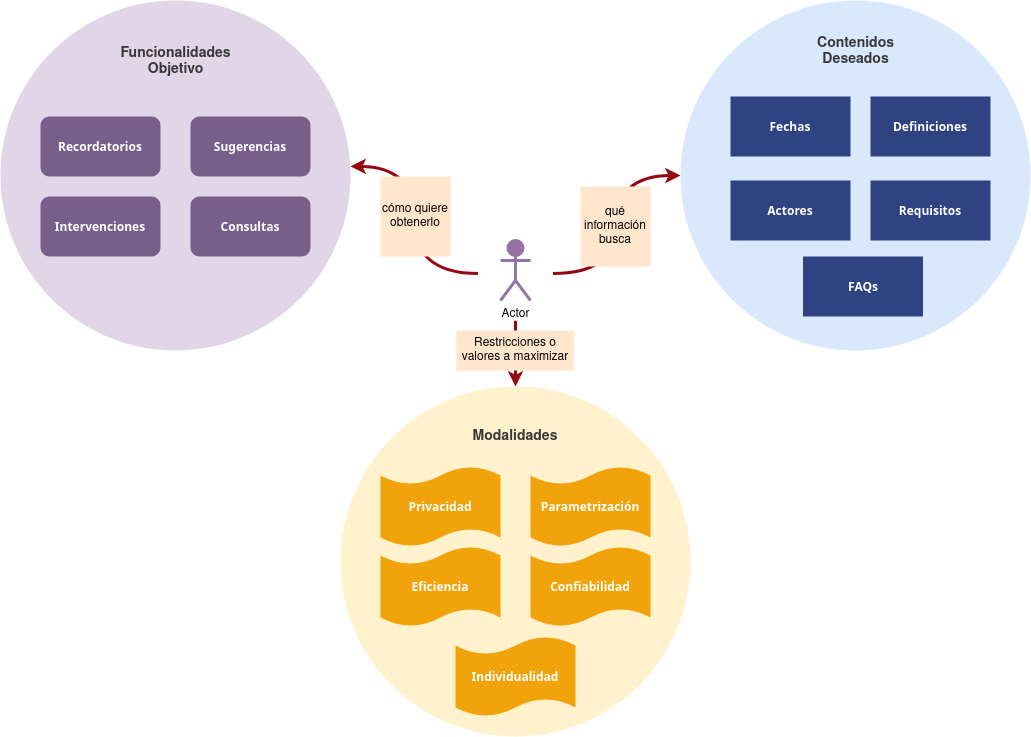
\includegraphics[scale=0.4]{media/imagenes/focus_groups/objetivos_y_cualidades.png}
        \caption{Diagrama que busca plasmar las superclases en las que se agrupan los objetivos de los alumnos a sí como las funcionalidades del sistema. Todo agrupado en categorías}
        \label{fig:my_label}
    \end{figure}

\section{Análisis de requisitos}
        \par Para poder plasmar nociones como seguridad, individualidad y personalización, es necesario interactuar varias veces con un cliente. Además, para que un diseño que integre visiones opuestas de lo que se requiere, es necesario plasmar alternativas diferentes de un mismo servicio. Estas complejidades se expresan y se detallan a través de diagramas i* (ver \ref{sec:intro-met}).
        \par Por lo tanto los siguientes diagramas plasman las preferencias de los usuarios obtenidas de los \acrlong{f}, y permiten el diseño y discusión del proceso cómo un todo. Este proceso simplifica el diseño general y permite que la discusión se centre en lo que se requiere lograr y cómo lograrlo, y no en cada camino para llegar a ello específicamente. Es decir se mantiene un alto nivel de diseño.
        \par A continuación se explican las funcionalidades y objetivos esperados por los usuarios, a través de 4 diagramas Consultas, Intervenciones, Recordatorios y Sugerencias.
    
    \subsubsection{Consultas}
        \begin{figure}[ht]
            \centering
            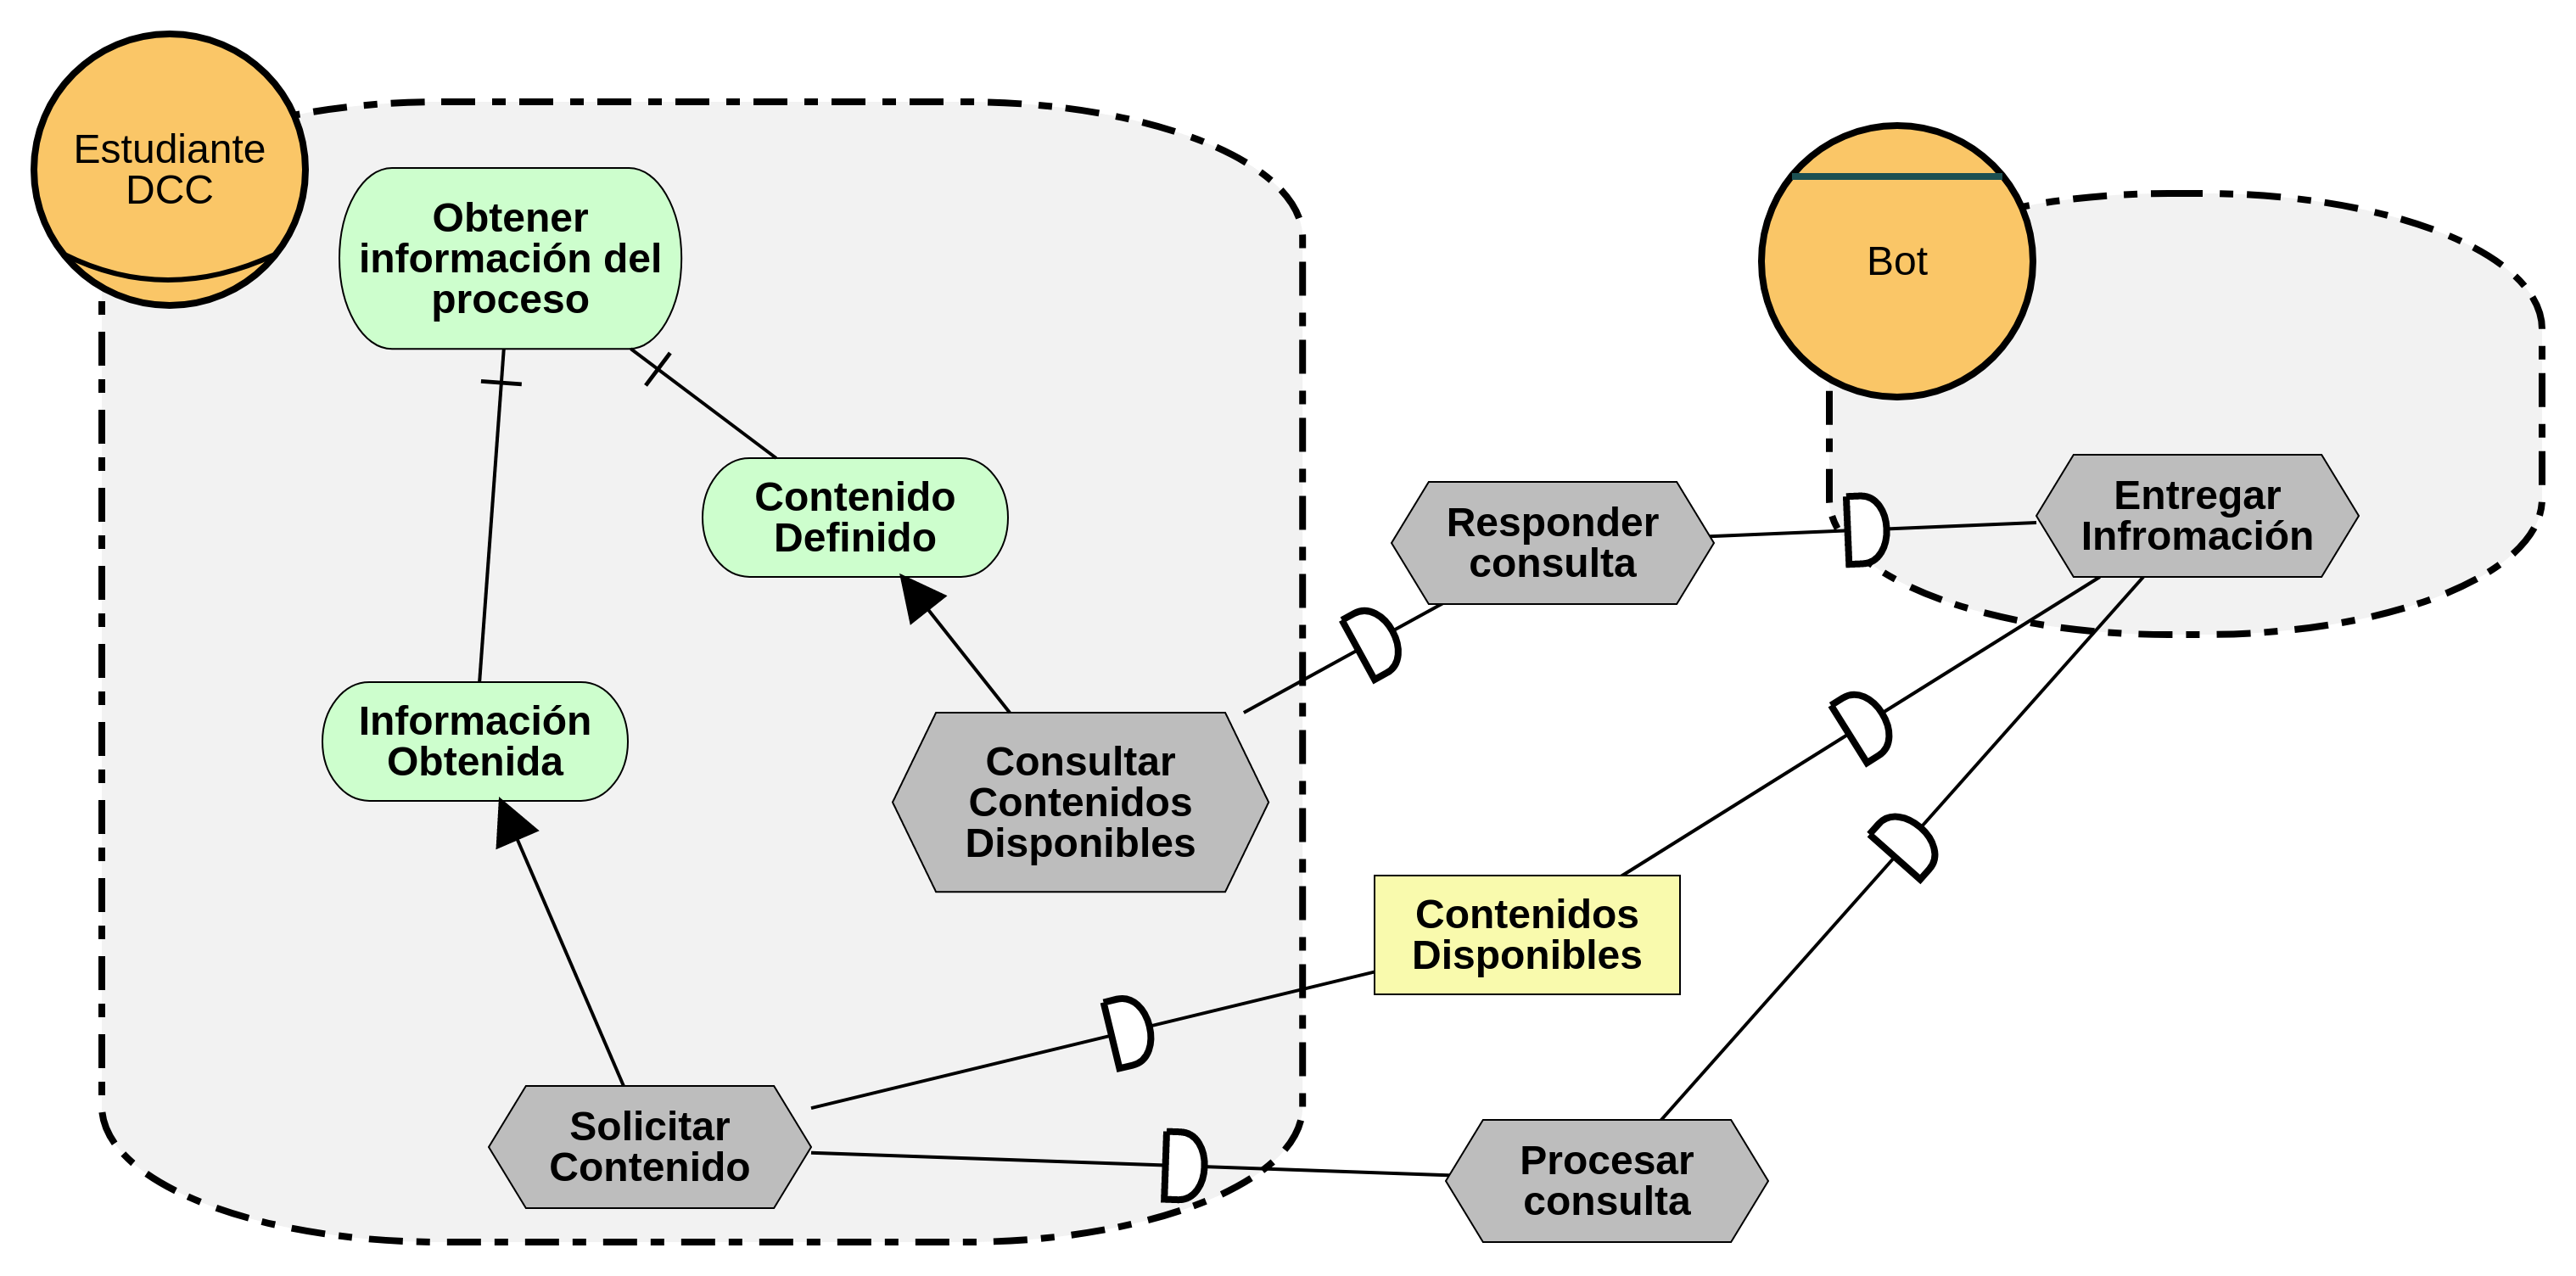
\includegraphics[width=\textwidth]{media/imagenes/i_star/diagramas/Consultas.png}
            \caption[Diagrama i* Consultas]{Diagrama que representa la consulta por información}
            \label{}
        \end{figure}

        \par Una de las principales necesidades de los estudiantes en torno a los procesos académicos y administrativos es obtener información, en el diagrama esquematizamos este proceso. 
        \par Cómo se puede observar el objetivo principal del estudiante del dcc (en esta interacción) es Tener información del proceso.
        \par Para Conseguir información, debe cumplir  con tener un contenido definido, y con haber sido informado (o estar informado).
        \par Ahora para lograr esto, el usuario debe solicitar un contenido al bot, quien procesara la consulta, luego entregará el contenido disponible y el alumno podrá seleccionar que contenido desea conocer, a lo que el bot ayudará a completar respondiendo la información por el proceso seleccionado.Esta interacción simple en dos pasos, engloba varias funcionalidades especificas. Por ejemplo los contenidos se entregan y consultan de formas diferentes. También hay ciertos contenidos que se requieren con más o menos frecuencia. Sin embardo como se puede observar, este diagrama representa lo que se quiere lograr y cómo lograrlo a modo general.
        \par Esto permite un diseño lógico posterior de todas las funcionalidades que se comportan de manera similar puedan ser entendidas bajo el alero de esta descripción.
        \par Cómo veremos en detalle en la sección siguiente esto permite: Diseñar los diferentes mecanísmos con un ordén lógico y manteniendo siempre el foco en el problema. Por otro lado, permiten que la comunicación y extensión de funcionalidades similares se pueda explicar de forma sencilla a nuevos desarrolladores uno de los objetivos del proyecto. 
        \par Ejemplos de lo expresado son que por ejemplo el FAQ es una forma de consultar información. Otra modalidad de consultas también recae sobre este modelo, y a pesar de que un método use una vía de comunicación distinta, incluso ejecuten procesamientos de datos difenrentes, todos ellos responden a la misma funcionalidad, esto permite extender el esta área del sistema, aun estando bajo la lógica de retribuir información que el usuario consulta dentro de un catálogo
    
    \subsubsection{Recordatorios}
        \begin{figure}[ht]
            \centering
            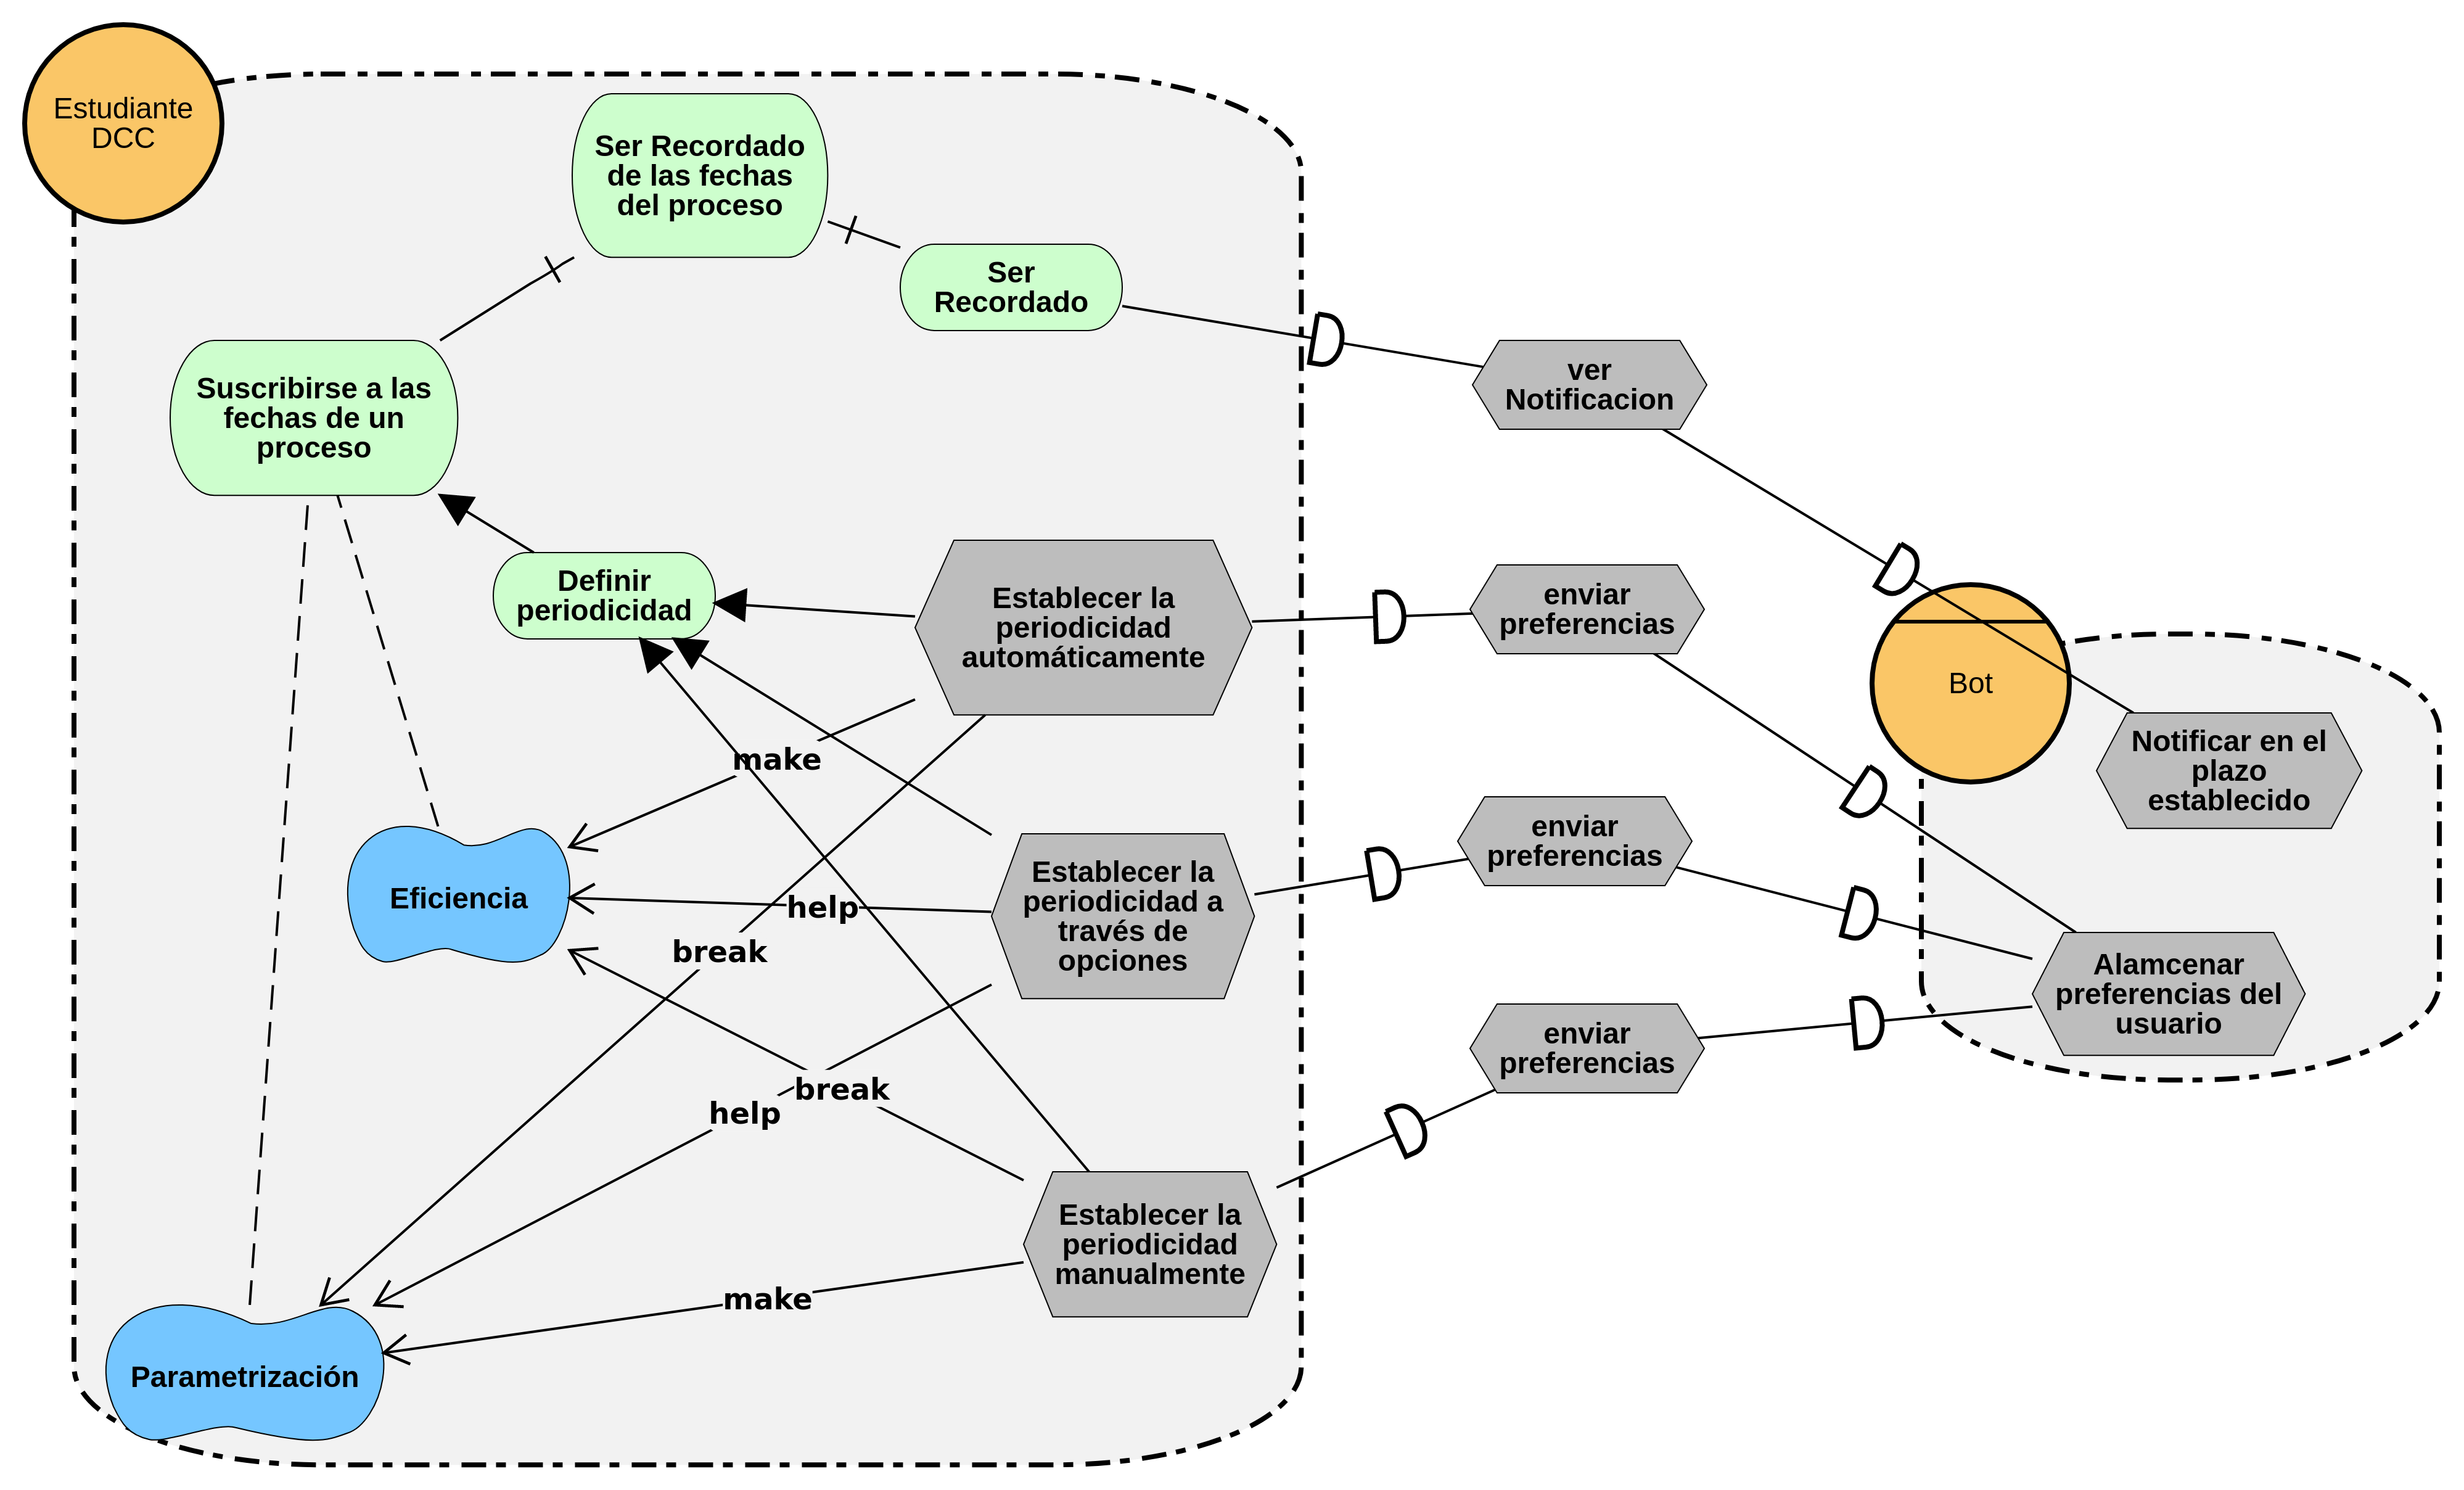
\includegraphics[width=\textwidth]{media/imagenes/i_star/diagramas/Recordatorios.png}
            \caption{}
            \label{}
        \end{figure}

        \par Otra de las funcionalidades que estudiamos fue la de ser recordados sobre las fechas de algún proceso académico. Cómo, por ejemplo, durante el proceso de titulación: la fecha para definir el tema, definir profesor guía, entregar el informe de propuesta, etc.

        \par A partir del análisis también se obtuvo que existían 2 cualidades o características que se valoran en cuanto a ser recordados, 1 es la eficiencia y otro es la parametrización (nota al pie: la definición de cada una se puede ver en la sección anterior). La eficiencia en este caso hace referencia a que si me suscribo a un recordatorio quiero que el sistema sepa como debo ser recordado, de forma de hacer el proceso simple, rápido y por sobre todo que me asegure el resituado. La parametrización, por otro lado, tiene que ver con establecer todos los parámetros que se consideren relevantes, cómo: Cuando soy notificado.

        \par En este sentido, los alumnos propusieron 3 maneras de establecer la periodicidad de una subscripción o recordatorios: automáticamente (el sistema define predeterminadamente cuando), a través de opciones predefinidas: 2 semanas, 1 mes, 1 día, etc., algo que aplicaciones como outlook o google calendar han recogido y permiten en sus sistemas.

        \par En el diagrama, si bien se puede observar que existen las tres alternativas favorecen de maneras diferentes las cualidades valoradas por los alumnos, si bien, por un lado, establecer la periodicidad manualmente hace que la aplicación sea parametrizable, la ha menos eficiente, el caso contrario ocurre al establecer la periodicidad automáticamente.

        \par Una de las conclusiones importantes que se saca de este diagrama es que tener las 3 alternativas es la única forma de favorecer a todos los usuarios de sistema en cuanto a sus preferencias. Sin embargo, eso implica desarrollar 3 vías adecuadas especialmente para ese objetivo.
        \par Otra conclusión interesante que se extrae de diagrama es que el bot, debe guardar una configuración específica para cada estudiante, en orden de favorecer las cualidades que son importantes para él. Si bien esto podría eventualmente ser un riesgo de privacidad, tanto desde lo extraído de los alumnos como lo la forma en que está creado el bot, hacen que se puedan guardar estas preferencias de forma anónima.
        \par Y finalmente, como es de esperarse, el bot debe ser capaz de notificar también en una fecha particular a cada alumno.
        \par Este diagrama, si bien en pocos pasos, da cuenta de una complejidad subyacente en torno a diseñar e implementar una funcionalidad puede hacer que un grupo de alumnos se vea favorecido y otro perjudicado, estas conclusiones son relevantes a la hora de priorizar o establecer metas de desarrollo.

    \subsubsection{Sugerencias}
        \begin{figure}[ht]
            \centering
            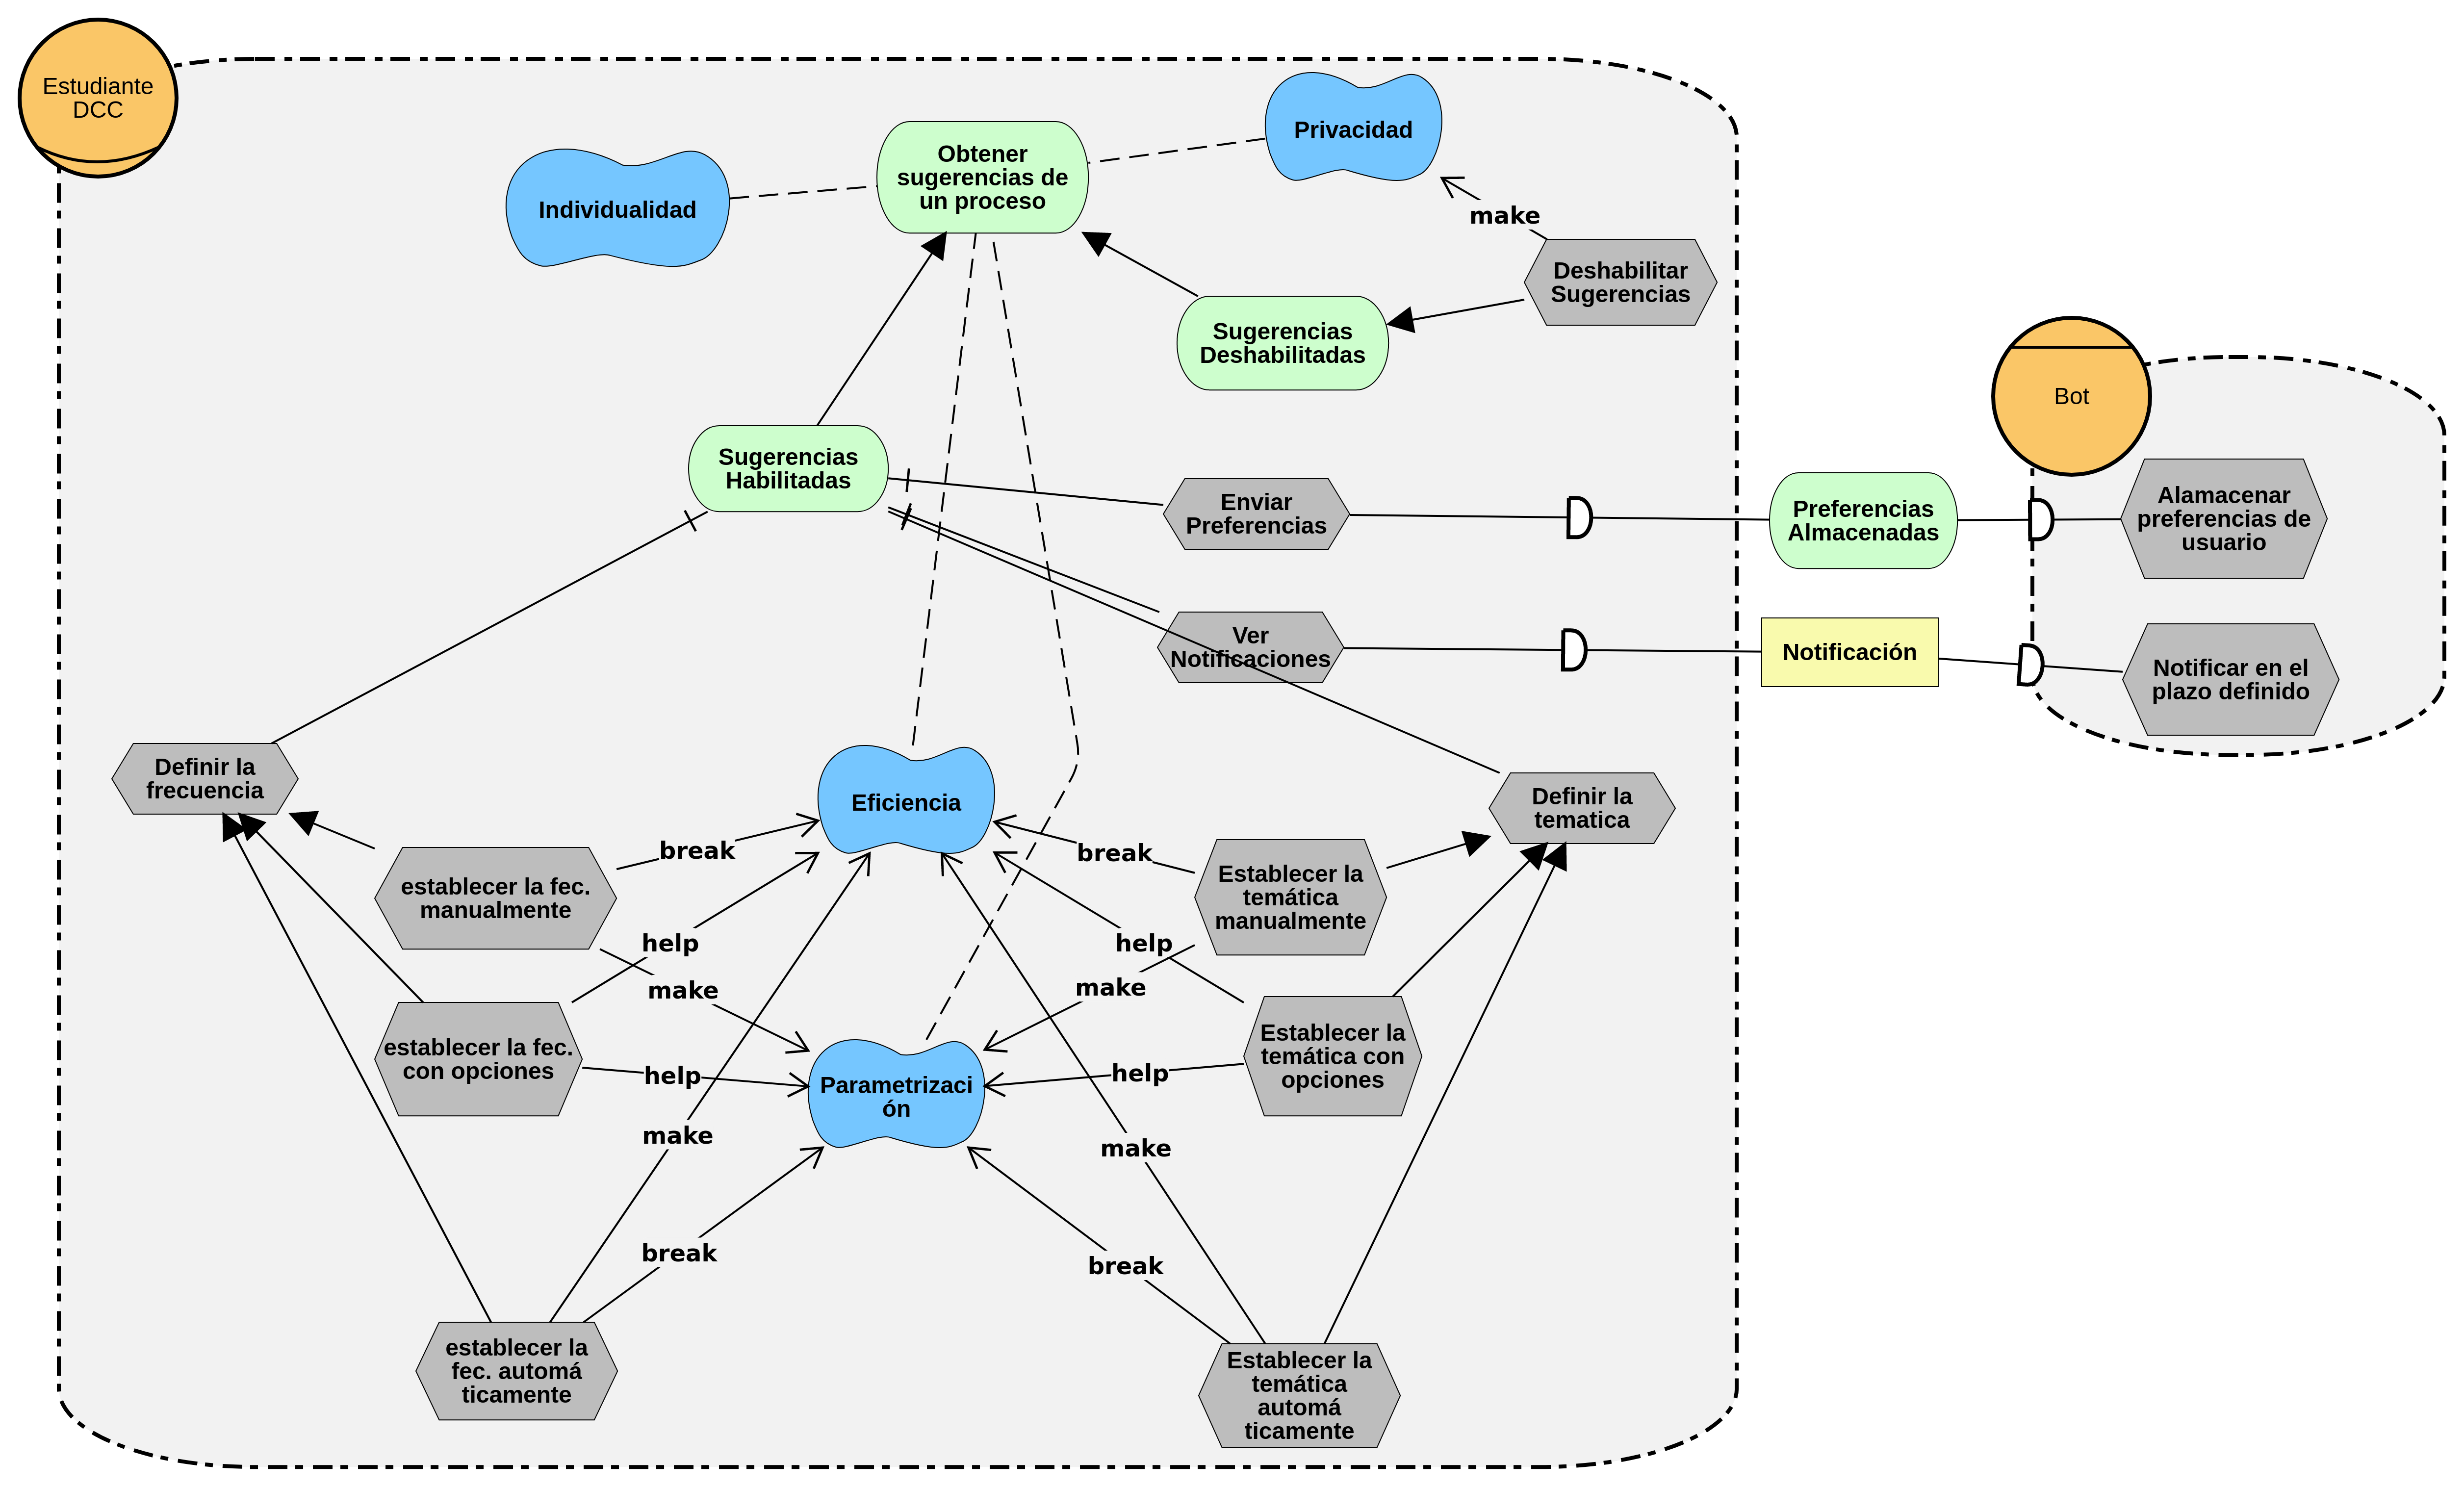
\includegraphics[width=\textwidth]{media/imagenes/i_star/diagramas/Sugerencias.png}
            \caption{}
            \label{}
        \end{figure}
        \par Las sugerencias son un tipo de funcionalidad pensada en alumnos que no tienen claro que deben hacer, se adelanta a las posibles dudas del alumno y entrega recomendaciones sobre alguna de las alternativas disponibles. Esta fue una de a las funcionalidades más contradictorias en términos de lo valorado por los alumnos y esto se puede observar en las cualidades adjuntas a esta funcionalidad.
        \par En primer lugar, este es un sistema particularmente individualizado, esto quiere decir que las sugerencias que son particularmente específicas a cada alumno, sobre todo porque algunos de lleno no quieren recibir sugerencias.
        \par Es una funcionalidad también que es recibida con un poco más de recelo por parte de los mismos estudiantes, porque para que el sistema pueda dar sugerencias debe tener más información de los alumnos, la que podría hacerlos identificables y con ellos las problemáticas que podrían surgir a partir de exponer las preferencias de cada uno.
        \par Al mismo tiempo, es extremadamente eficiente para un grupo de alumnos que hubieran querido más guía y asesoría en su proceso académico, sobre todo que alguien se adelantara a lo que les pudiera hacer falta y les avisara con tiempo.
        \par También se observa una discusión similar a los recordatorios en cuanto, a la parametrización y eficiencia.
        \par Ahora algo interesante, aunque muy similar a establecer los pla       \par Una consideración que hay que tener, es que en un proceso de análisis normal, usualmente se plantean como objetivos "tareas" a lograr y no estados a los que se quiere llegar, por lo tanto, es extraño definir un objetivo como por ejemplo: Tener el Contenido definido. Sin embargo, esto ayuda a ver que la tarea en si no es el objetivo final (que es un problema que traspasamos al diseño de software). 
        \par El objetivo no es la creación de un sistema que resuelva una tarea, sino que es la motivación para hacer un sistema que resuelva una tarea de software. En nuestro ejemplo, para tener información sobre un proceso, a la persona le debe surgir una inquietud, cuando eso ocurre, el estado al que se desea llegar es tener la información que conteste su inquietud. Así mismo, debe consultar para obtener esta información, pero eso es a partir de tener definido este contenido a consultar, usualmente, este proceso es automático y/o heurístico en el ser humano, por lo tanto es fácil tratar funcionalidades del sistema como objetivos del usuario, eso en general hace que se pierda de vista, la manera en que deben ser logrados estos objetivos, a la vez quezos, sin duda una de las cualidades clave de este sistema, sería establecer la temática de las sugerencias. Uno de los grandes problemas que el bot busca resolver, es el hecho de que a pesar de tener mucha información disponible, los alumnos continúan con dudas e incertidumbres. Esto debido a dos razones principales, 1 es el exceso de información no relevante y la otra el desconocimiento de los canales existentes. Un sistema que agrupe la información sería valioso para solucionar el problema de tener múltiples canales, y una mejora significativa en la experiencia se daría si los alumnos reciben información que es importante para ellos y no cualquier cosa.
        \par Esta es una discusión particularmente especial, porque es similar a las disyuntivas que presenta el desarrollo de redes sociales, y este aspecto del bot se ve muy influenciado por las percepciones que los alumnos tienen de las políticas establecidas en cada una de ellas.

    \subsubsection{Intervenciones}
        \begin{figure}[ht]
            \centering
            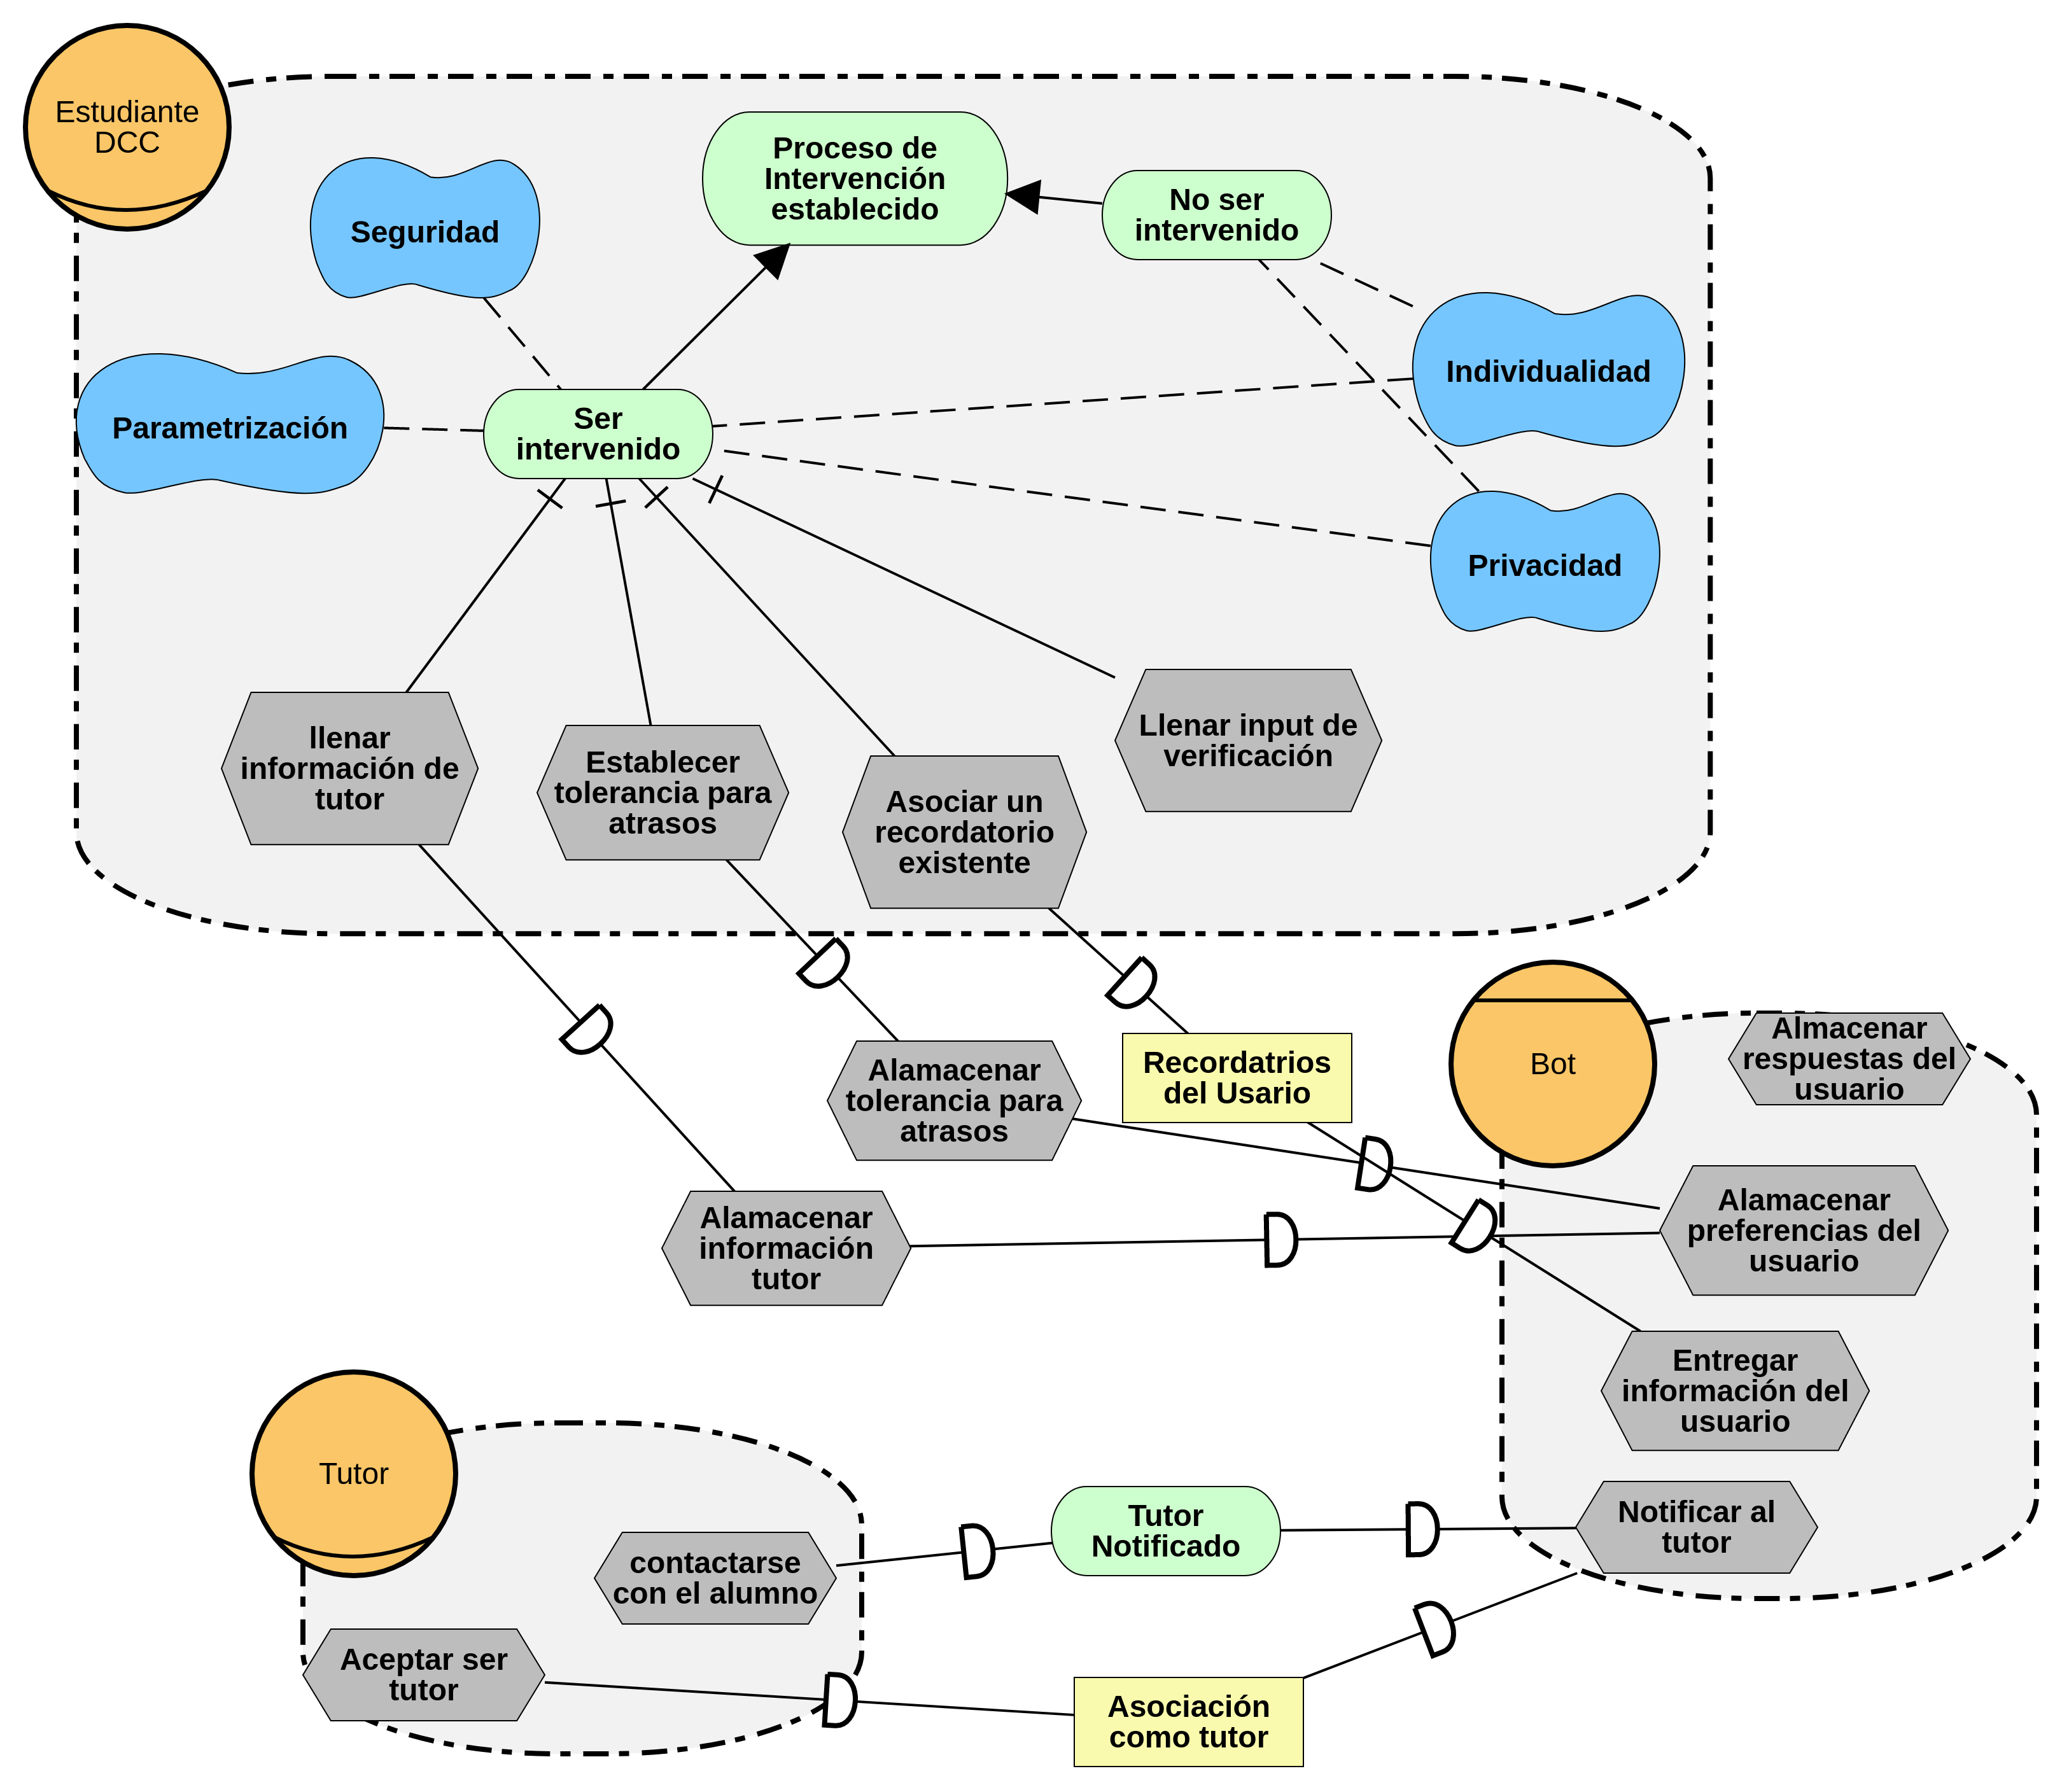
\includegraphics[width=\textwidth]{media/imagenes/i_star/diagramas/Intervenciones.png}
            \caption{}
            \label{}
        \end{figure}
        \par Las intervenciones, soporte o tutelaje tienen el objetivo de incluir a un tercero en el recorrido del alumno por un proceso, y que este pueda ser una voz amigable para revisar el estado del proceso. Este “Tutor” cómo se denomina, es notificado cuando el alumno no interactúa con los elementos a los que el mismo se suscribió, esta funcionalidad, busca que el alumno pueda recibir apoyo cuando por diversas razones podría no estar dándole la atención necesaria al proceso. Esta funcionalidad, al igual que las sugerencias, se adelanta a que el alumno pudiese tener un problema o atrasarse en los plazos.
        \par Cómo se puede ver en el diagrama, las cualidades de individualidad y privacidad son factores determinantes a la hora de decidir si usar o no esta funcionalidad. Por otro lado la tranquilidad que puede brindar al estudiante el tener un soporte externo que puede ser cualquier persona, es uno de los mayores incentivos para agregar esta feature.
        \par Otra de las razones por las que puede ser controversial es porque debe almacenar interacciones del alumno en el sistema, se deben guardar contactos de terceros, etc.

\section{Conclusiones generales de Análisis}
    \par A modo general, desde los diagramas se pueden obtener varias nociones que pueden guiar el trabajo. Se presentan las funcionalidades a realizar por el sistema en las tareas que deben realizar los distintos agentes involucrados (hexagonos grises). Y, por otro lado, las cualidades vienen a ser restricciones y alternativas a las mismas funcionalidades. También algunos de los contenidos quedan explícitos como recursos (rectángulos amarillos). Así mismo todos los actores relevantes para una funcionalidad. Siempre teniendo a la vista cuál es el objetivo final de cada una de las funcionalidades globales.
    
    \par Una consideración que hay que tener, es que en un proceso de análisis normal, usualmente se plantean como objetivos \guillemotleft tareas \guillemotright a lograr y no estados a los que se quiere llegar, por lo tanto, es extraño definir un objetivo como por ejemplo: Tener el Contenido definido. Sin embargo, esto ayuda a ver que la tarea en sí, no es el objetivo final (que es un problema que traspasamos al diseño de software). 
    \par El objetivo no es la creación de un sistema que resuelva una tarea, sino que es la motivación para hacer un sistema que resuelva una tarea de software. En nuestro ejemplo, para tener información sobre un proceso, a la persona le debe surgir una inquietud, cuando eso ocurre, el estado al que se desea llegar, es tener la información que conteste su inquietud. Así mismo, debe consultar para obtener esta información. Pero, eso es a partir de tener definido este contenido a consultar. Usualmente, este proceso es automático y/o heurístico en el ser humano, por lo tanto es fácil tratar funcionalidades del sistema, como objetivos del usuario. Eso en general hace que se pierda de vista, la manera en que deben ser logrados estos objetivos.
        
    \par Este tipo de análisis, permite distinguir entre los requisitos de usuarios (objetivos y cualidades) y los requisitos de software (tareas, recursos y cualidades) de manera global, muy útil en la dirección estratégica de proyectos. Mantener este tipo de nociones resulta fundamental en el desarrollo orientado a usuarios, porque es muy fácil que el quehacer del proyecto se puedan perder los horizontes originales y perder de vista el objetivo por el cual se desarrolla el sistema.
    \par Por otra parte, hay que notar que estos diagramas representan un escenario ideal. En el que se extraen las necesidades, objetivos y restricciones de manera explícita en el planteamiento de una solución. Pero como todo desarrollo de software, se deben priorizar las funcionalidades de mayor importancia y también las que sean alcanzables durante la implementación. Respetando las reglas tiempo de todo desarrollo.
    \par Desde del análisis del \acrlong{f}, de los diagramas, y el traspaso del trabajo anterior, Se puede establecer a modo general, cuáles son los principales requerimientos. Estos debieran serán los que se alinean mejor con los objetivos de: \guillemotleft extender el sistema actual, agregando funcionalidades que permitan crear un sistema extensible, personalizado y confiable.\guillemotright Considerando la complejidad de implementación se opta por: Las consultas y recordatorios. 
    \par Ambos agregan valor deseado por los usuarios, permiten personalizar su experiencia en cuanto a la información que desean conocer y son los que presentan la mayor aceptación en torno a privacidad y otras cualidades valoradas por los usuarios.
    \par También se hace necesario analizar y modificar el sistema existente, para que sea capaz no solo de cumplir con la funcionalidad esperada, sino ser extensible de manera lógica y garantizar el desarrollo continuo de la plataforma.

\section{Diseño de plataformas}
    A partir de los requerimientos recabados en el trabajo anterior, se diseñaron varios diagramas UML, que permitieron esquematizar las principales funcionalidades y cambios a realizar en el sistema. Eso sí, es fundamental decir que a estos diseños sufrieron modificaciones durante el transcurso del proyecto y algunos como el diagrama de objetos obtiene su versión final en el modelo de datos. La versión de los diseños que se presenta aquí es la obtenida a partir del análisis de los requerimientos y el planteamiento incial.

    \subsection{Diseñar los casos de uso a partir de los objetivos de Usuario}
    \par Los casos de uso, son posibilidades que el sistema da a los usuarios. En nuestro diseño, representan funcionalidades de las que los estudiantes pueden hacer uso. Traspasando la notación \gls{i*}, los casos de uso vendrían a ser cada una de las maneras en que se cumple un objetivo, en otras palabras funcionalidad = Tarea a realizar.
    \par Los casos de uso considerados son los siguientes.

        img Casos DE USO

    \par Durante el planteamiento de los casos de uso, se agruparon varias de las tareas. Sobre todo porque desde los diagramas se extrae que: si bien el contenido puede variar, la funcionalidad deseada es la misma.
    En resumen del diagrama se puede extraer que el alumno podrá hacer 3 cosas principalmente en el sistema: Buscar información, suscribirse a información y habilitar permisos.
    \par Cada una de estas funcionalidades clave, tiene muchos pasos y diseños asociados, por eso se mostrará a continuación el diagrama de estados de una de ellas, a modo de ejemplo. Se eligió el digrama de estado del proceso de susbcripción porque es una de las interacciones más abarcantes y representativas del sistema, y permite ver cómo interactua el usuario con la información y cómo responde el sistema.

        img DIagrama de estados
            

    \par En la figura anterior, se puede observar que el alumno debe seleccionar primero un proceso vigente y a partir de ahí, seleccionar alguno de los contenidos disponibles. Definido esto, se procede a elegir la funcionalidad deseada en torno al contenido y finalmente se solicita al alumno aceptar o no el almacenamiento de los datos, equivalente a permitir o rechazar la funcionalidad. 
    \par Una salvedad es que si los permisos hubieran sido aceptados en el pasado o configurados globalmente, se puede pasar directamente a la funcionalidad esperada en este caso los recordatorios.
    \par Una de las principales conclusiones de este diseño (que es que un diseño basado en una interfaz), es que necesariamente consta de varios pasos. Los cuales se pueden simplificar y trabajar, pero añade muchas permutaciones en torno a los posibles viajes del usuario, y también tiene un alto costo de diseño. A sí mismo, si además de establecer este viaje \textit{default} agregamos la opción de que el usuario pueda parametrizar la frecuencia, se añaden muchas opciones de interfaz, lo que termina haciendo al sistema engorroso y lento de usar. Algo que no buscan los usuarios.
    \par Es por esto, que luego del diseño UML de varias de las plataformas, se diseñaron dos formas paralelas de acceder a las funcionalidades, para mantener la simplicidad y la eficiencia, por un lado, mientras que la parametrización y control sobre otro.
    \par Diseño Dual de interfaces y comandos
    Uno de los grandes hallazgos del proceso de diseño, es que las interfaces no se podían comportar de forma dual (eficiente y parametrizable), ya que se habrían tenido que añadir una gran cantidad de opciones de ajuste, esto al final redunda en un viaje de usuario muy largo, lo que claramente perjudica a los alumnos de tipo P.
    \par A partir de esto entonces se propuso un nuevo sistema que funciona de manera paralela a las interfaces basadas en botones y es una basada en comandos.
    Los comandos son una función bastante común en Telegram, ya que la mayoría de los bots ofrece un funcionamiento basados en comandos, esto permite no solo identificar una opción a realizar, sino que agregar en el mismo comando texto y valores que pueden servir cómo parámetros para dichas funciones. Este tipo de interfaz, más parecido a una shell o terminal, es bastante familiar para los alumnos del dcc y además usuarios de Telegram, en ese mismo sentido proporcionan una enorme flexibilidad y extensibilidad, dado que a partir de un mismo identificador se pueden efectuar muchos ajustes y configuraciones.

    % \subsubsection{Diagrama de comandos}

    \subsubsection{Diagrama de objetos}

    \par A partir de los casos de usos se creó el siguiente diagrama de objetos que da cuenta de las principales relaciones entre los objetos del sistema.Uno de los grandes cambios al modelo de original es la creación de un Usuario (o perfil) que debe servir como el centro para las suscripciones, los permisos y el usuario de apoyo. Así mismo se identifica que deben agregarse tablas de contenido para las instancias. Finalmente, una de las grandes modificaciones es que se necesita una forma de mantener un catálogo de las cosas a las que los usuarios pueden acceder, particularmente suscribirse, las que no pueden quedar simplemente en el código, ya que por naturaleza son mutables de instancia a instancia, eso implicaría agregar muchas líneas de código o quitar muchas para cada instancia de cada proceso en particular.
    \par El problema principal con este catálogo, es que se debe diseñar alguna forma de mantenerlo actualizado, por ahora el diseño es manual, pero en un futuro podría ser de forma automática.

    \subsection{Modelo de datos}
    \begin{itemize}
        \item User: Información de acceso al sistema de administración.
        \vspace{3mm}
        \par \textit{Relativos al Proceso}
        \item Proceso: Contiene los procesos que existan. Ejs: Proceso de Titulación, Prácticas, etc.
        \item Categorías: Categorías de las preguntas frecuentes.
        \item FAQ: Preguntas Frecuentes.
        \vspace{3mm}
        \par \textit{Relativos  a una instancia}
        \item Instancias: Instancias de un proceso, por ejemplo: Proceso de Titulación 2022.
        \item Novedades: Son las noticias, pero relacionadas a una instancia en particular del proceso.
        \vspace{3mm}
        \par \textit{Usuarios del Bot}
        \item Usuarios del Bot: identificador del chat.
        \item Permisos de los Usuarios del Bot: Configuraciones de funcionalidad y seguridad de los usuarios.
    \end{itemize}
    
    